% !TEX TS-program = xelatex
% !TEX encoding = UTF-8
% !Mode:: "TeX:UTF-8"

\documentclass[onecolumn,oneside]{SUSTechHomework}

\usepackage{float}

\author{胡玉斌}
\sid{11712121}

\title{Lab 10}
\coursecode{CS315}
\coursename{Computer Security}

\begin{document}
  \maketitle

  \section*{Task 1}

  We calculate the exgcd: $e \times d + \phi(n) \times y = 1$

  The Figure \ref{fig1} show how to calculate by python with \verb|sympy| package.

  d = 0X3587A24598E5F2A21DB007D89D18CC50ABA5075BA19A33890FE7C28A9B496AEB.

  \begin{figure}[H]
    \centering
    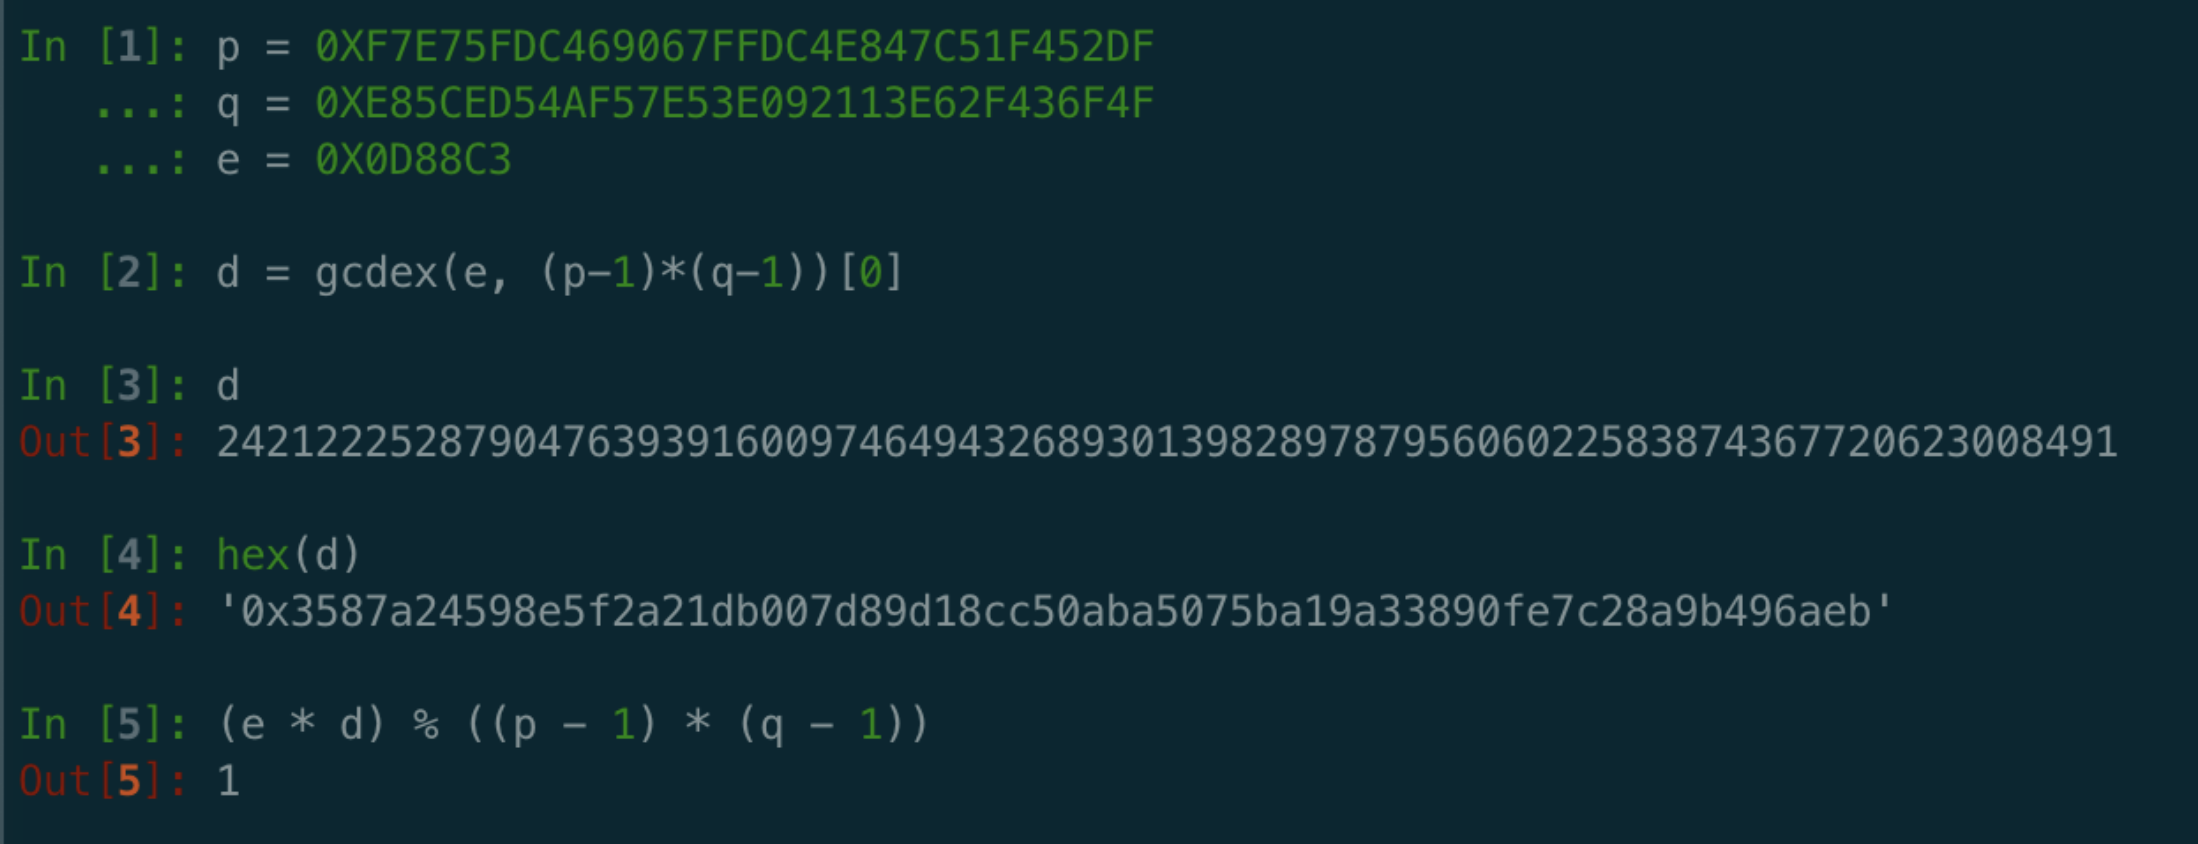
\includegraphics[width=0.85\textwidth]{img/task1_1.png}
    \caption{exgcd}
    \label{fig1}
  \end{figure}

  \section*{Task 2}

  Encrypting the message with RSA to calculate $C = M^e$.

  $C = \mbox{0X6FB078DA550B2650832661E14F4F8D2CFAEF475A0DF3A75CACDC5DE5CFC5FADC}$

  To verify that, calculate $M=C^d~\mbox{mod}~n$.

  \begin{figure}[H]
    \centering
    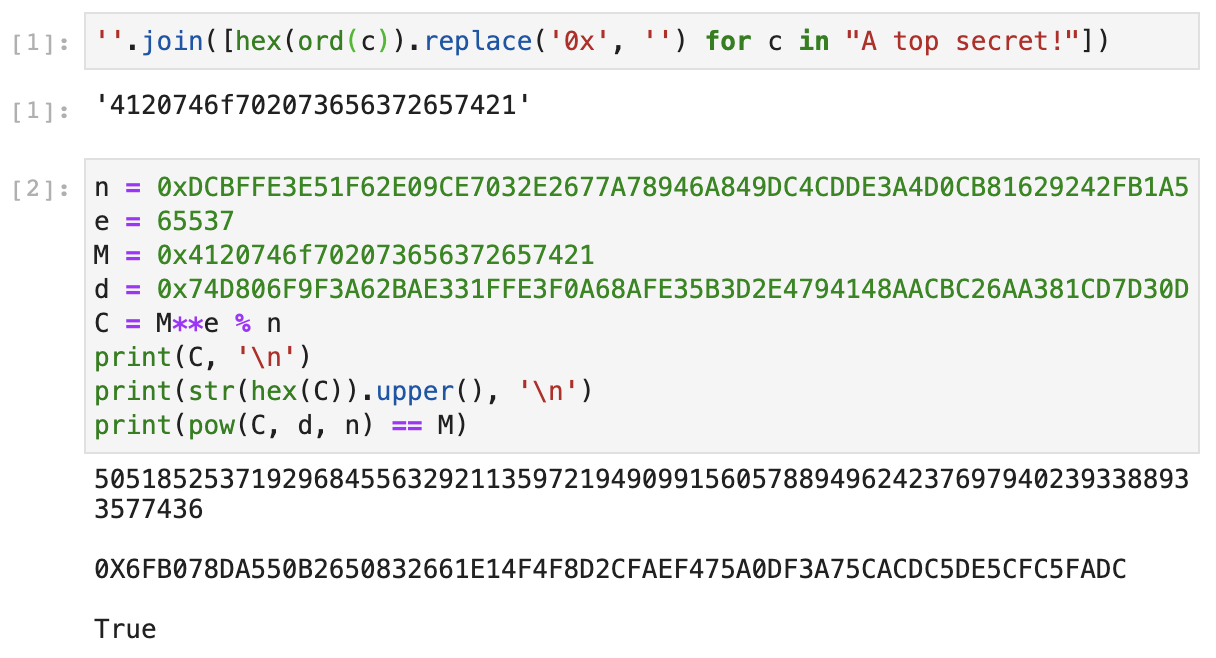
\includegraphics[width=0.85\textwidth]{img/task2_1.png}
    \caption{Encrypt}
  \end{figure}

  \section*{Task 3}

  Calculate $C^d$, we have $M = 0X50617373776F72642069732064656573$

  Decode by \verb|utf-8|, we get message \verb|Password is dees|

  \begin{figure}[H]
    \centering
    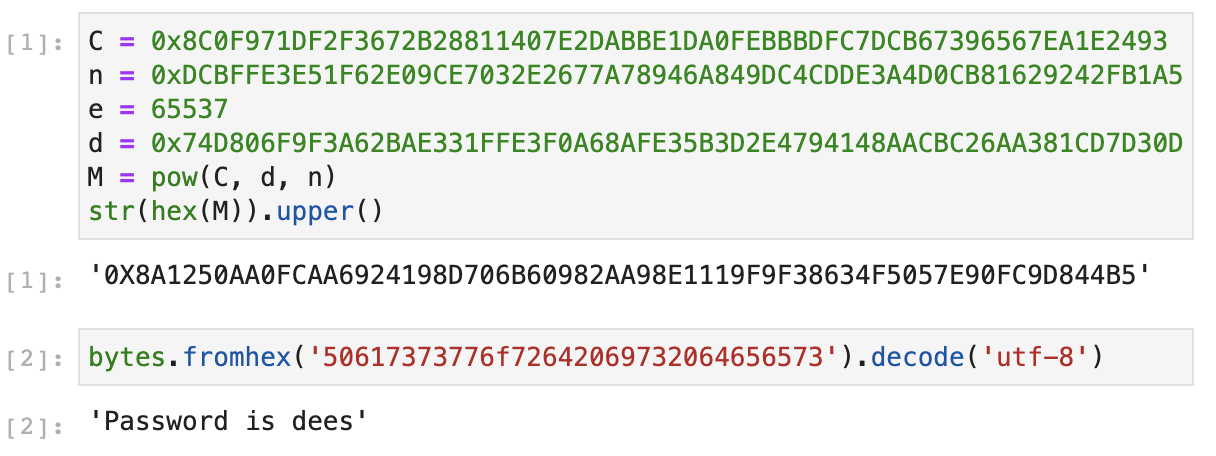
\includegraphics[width=0.85\textwidth]{img/task3_1.png}
    \caption{Decrypt}
  \end{figure}

  \section*{Task 4}

  We sign the message by calculating $S=M^d$

  We get $S=0X55A4E7F17F04CCFE2766E1EB32ADDBA890BBE92A6FBE2D785ED6E73CCB35E4CB$ when $M=\mbox{I owe you \$2000.}$

  We get $S=0XBCC20FB7568E5D48E434C387C06A6025E90D29D848AF9C3EBAC0135D99305822$ when $M=\mbox{I owe you \$3000.}$

  Although we change \verb|2000| to \verb|3000|, the signature $S$ is changed a lot.

  \begin{figure}[H]
    \centering
    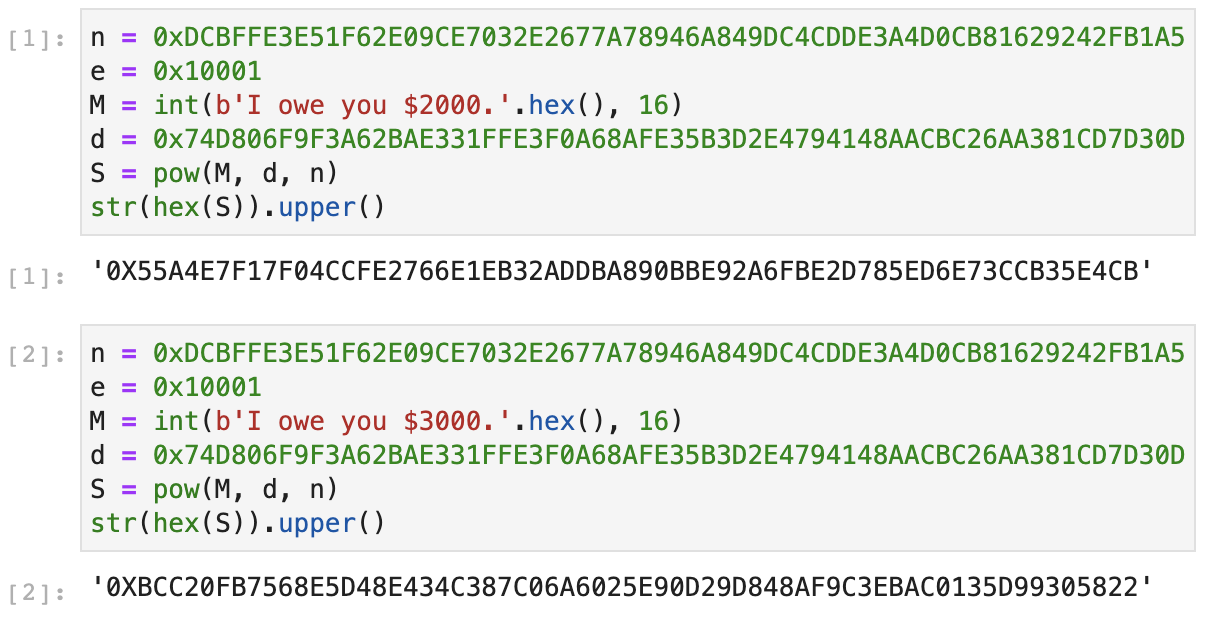
\includegraphics[width=0.85\textwidth]{img/task4_1.png}
    \caption{Sign}
  \end{figure}

  \section*{Task 5}

  If the signature is correct, sigen message is the same as actual message.

  But it the signature is wrong, the message is changed.

  \begin{figure}[H]
    \centering
    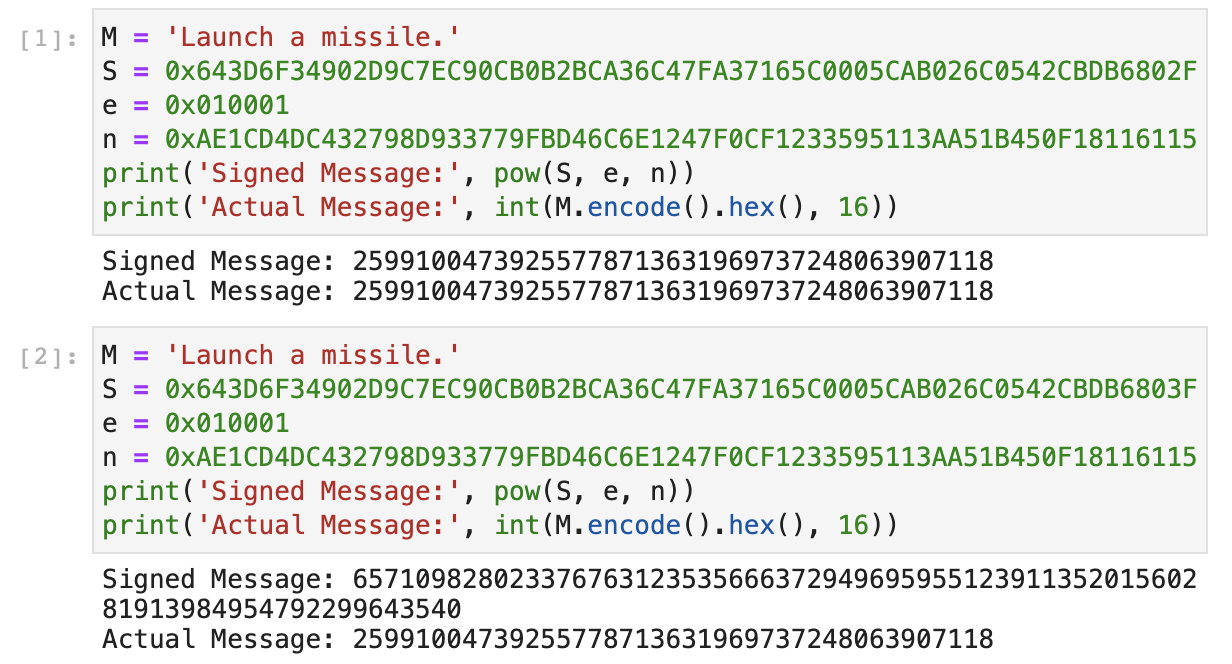
\includegraphics[width=0.85\textwidth]{img/task5_1.png}
    \caption{Verify}
  \end{figure}

  \section*{Task 6}

  \subsection*{Step 1}
  
  Download a certificate from a real web server.

  We use the \verb|www.baidu.com| server.

  \begin{figure}[H]
    \centering
    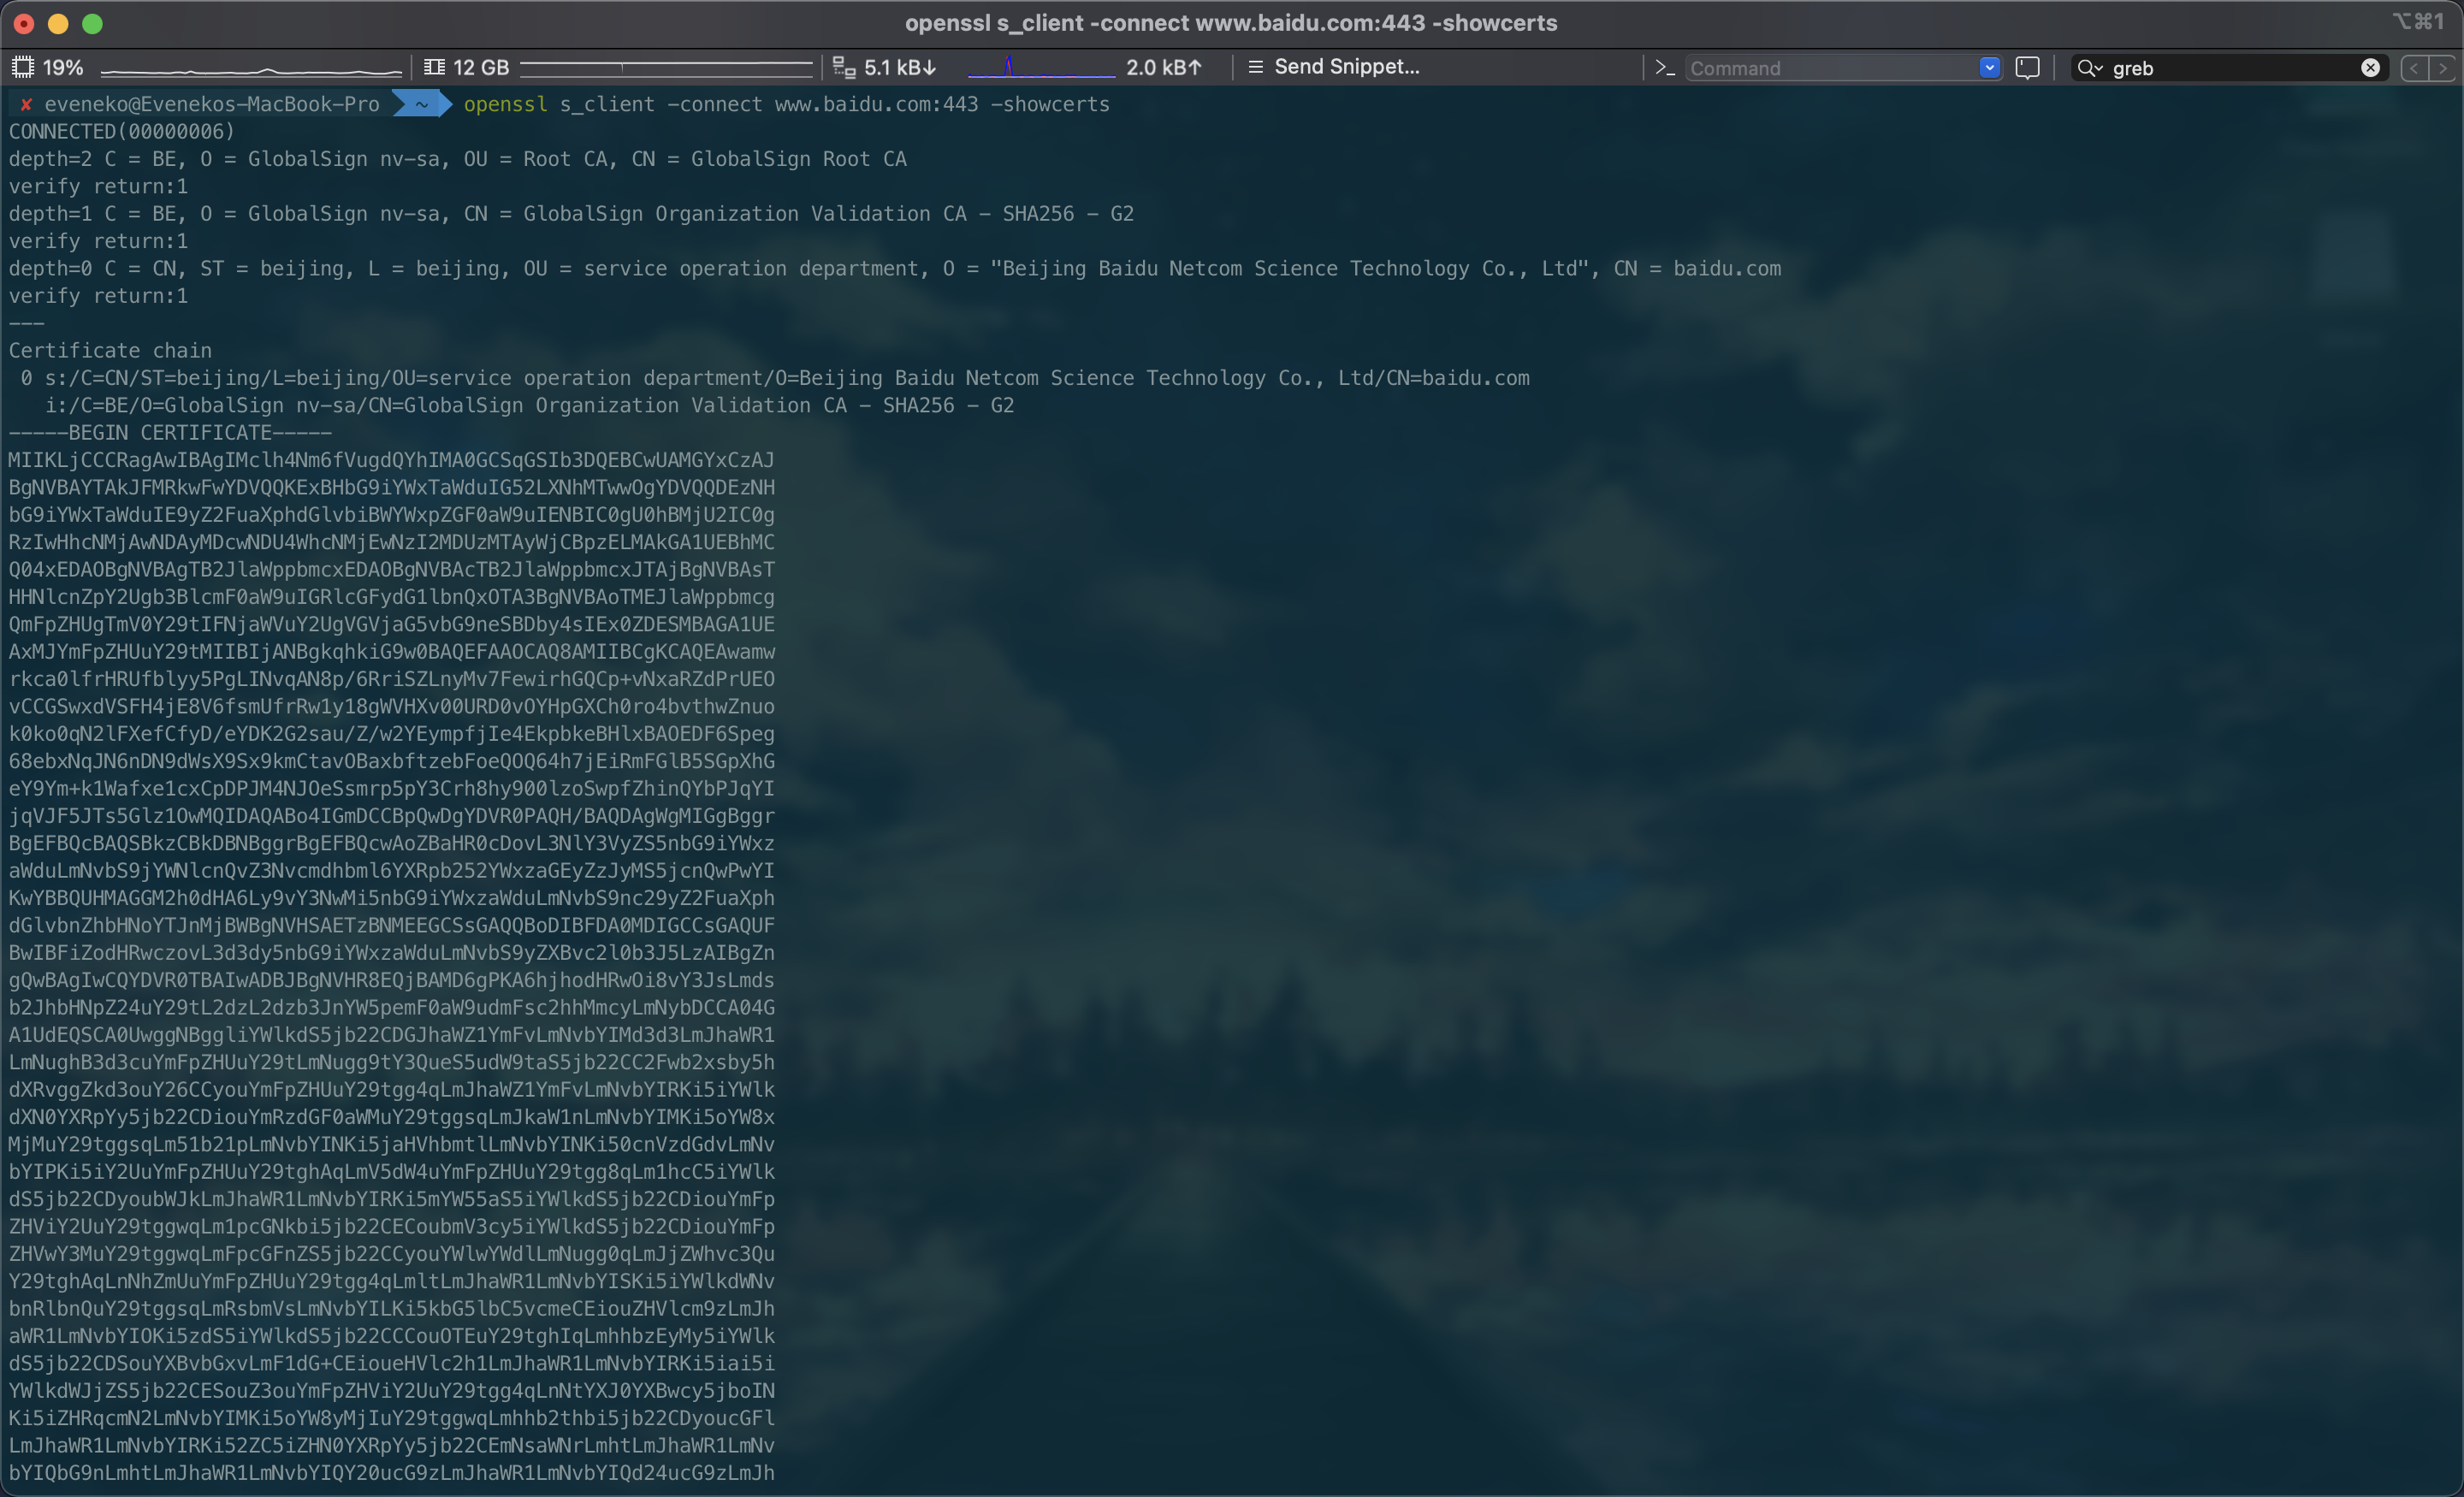
\includegraphics[width=0.85\textwidth]{img/task6_1.png}
    \caption{Step 1}
  \end{figure}

  \begin{figure}[H]
    \centering
    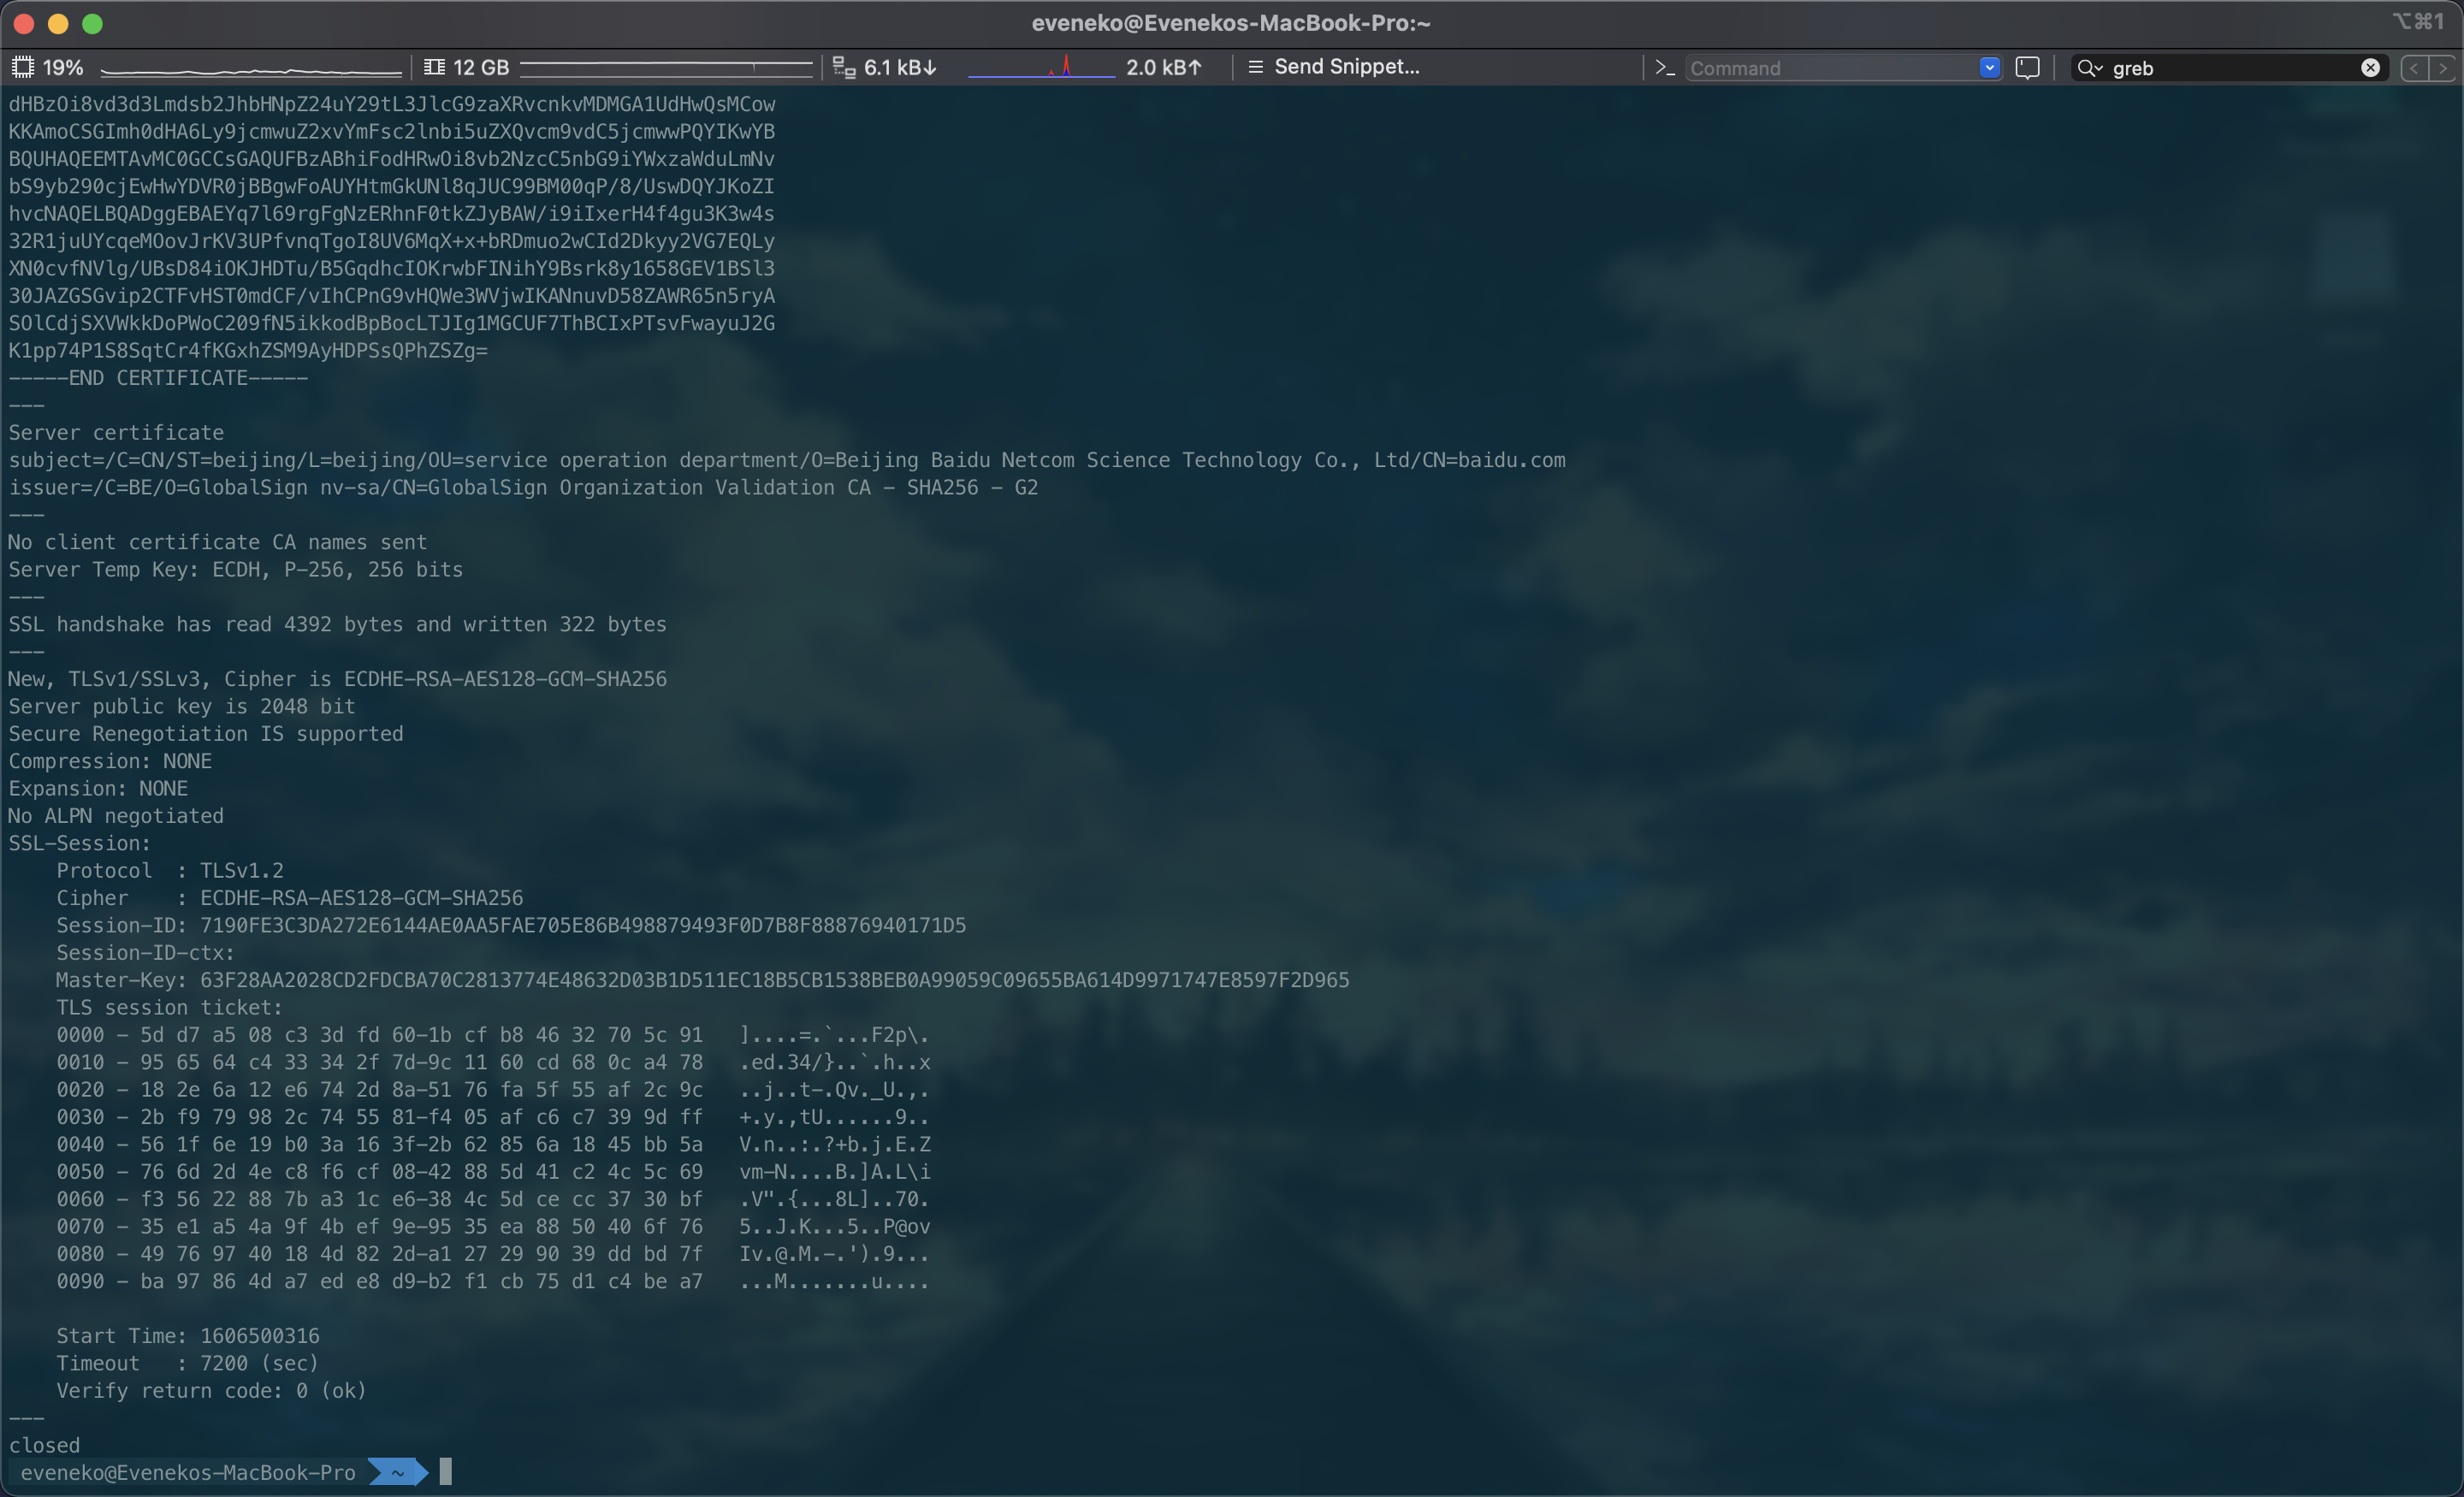
\includegraphics[width=0.85\textwidth]{img/task6_2.png}
    \caption{Step 1}
  \end{figure}

  \subsection*{Step 2}

  Extract the public key (e, n) from the issuer’s certificate.

  We have $n$ and $e=0x10001$ now.

  \begin{figure}[H]
    \centering
    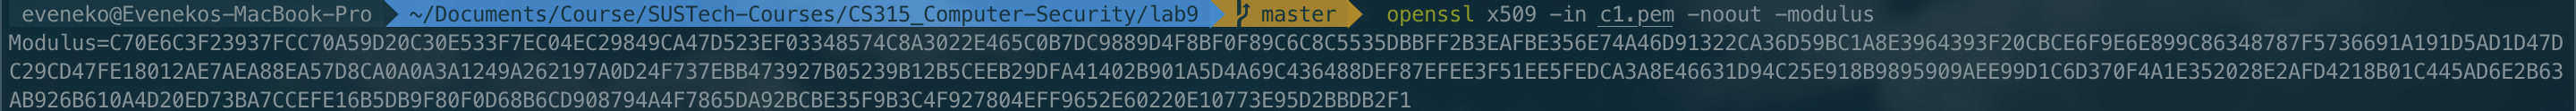
\includegraphics[width=0.85\textwidth]{img/task6_3.png}
    \caption{Step 2}
  \end{figure}

  \begin{figure}[H]
    \centering
    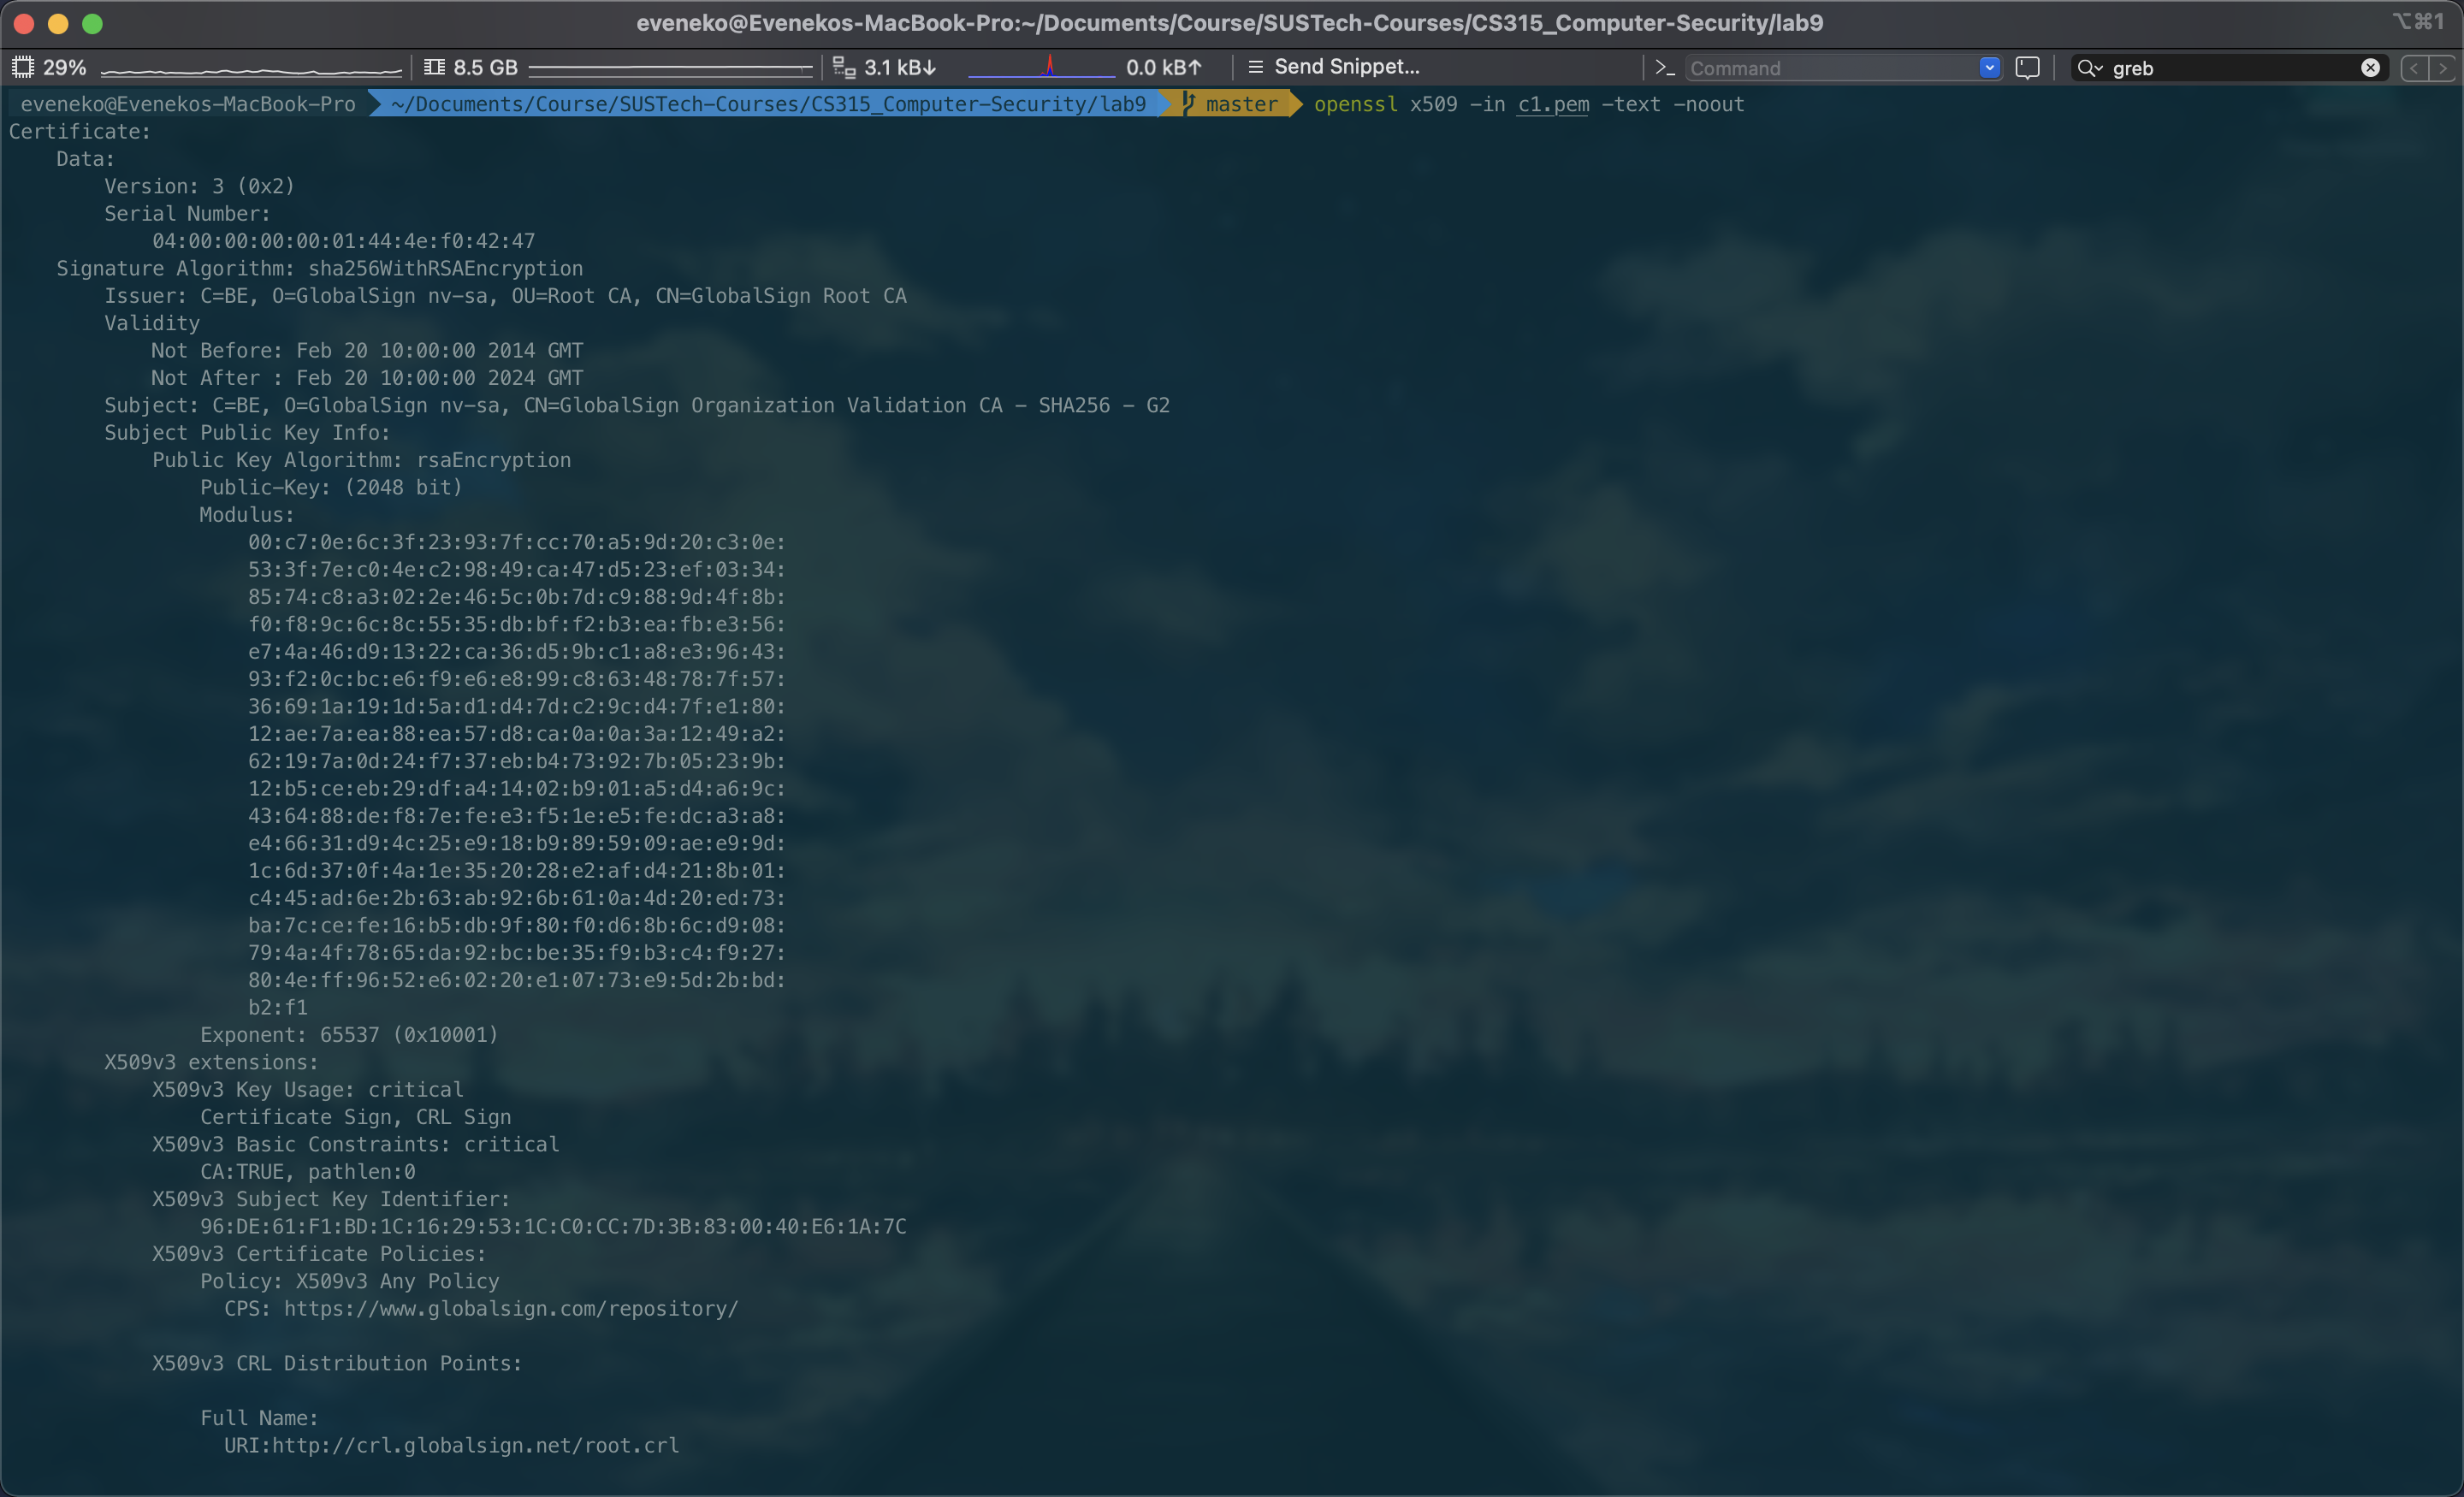
\includegraphics[width=0.85\textwidth]{img/task6_4.png}
    \caption{Step 2}
  \end{figure}

  \subsection*{Step 3}

  Extract the signature from the server’s certificate.

  We have $s$ now.

  \begin{figure}[H]
    \centering
    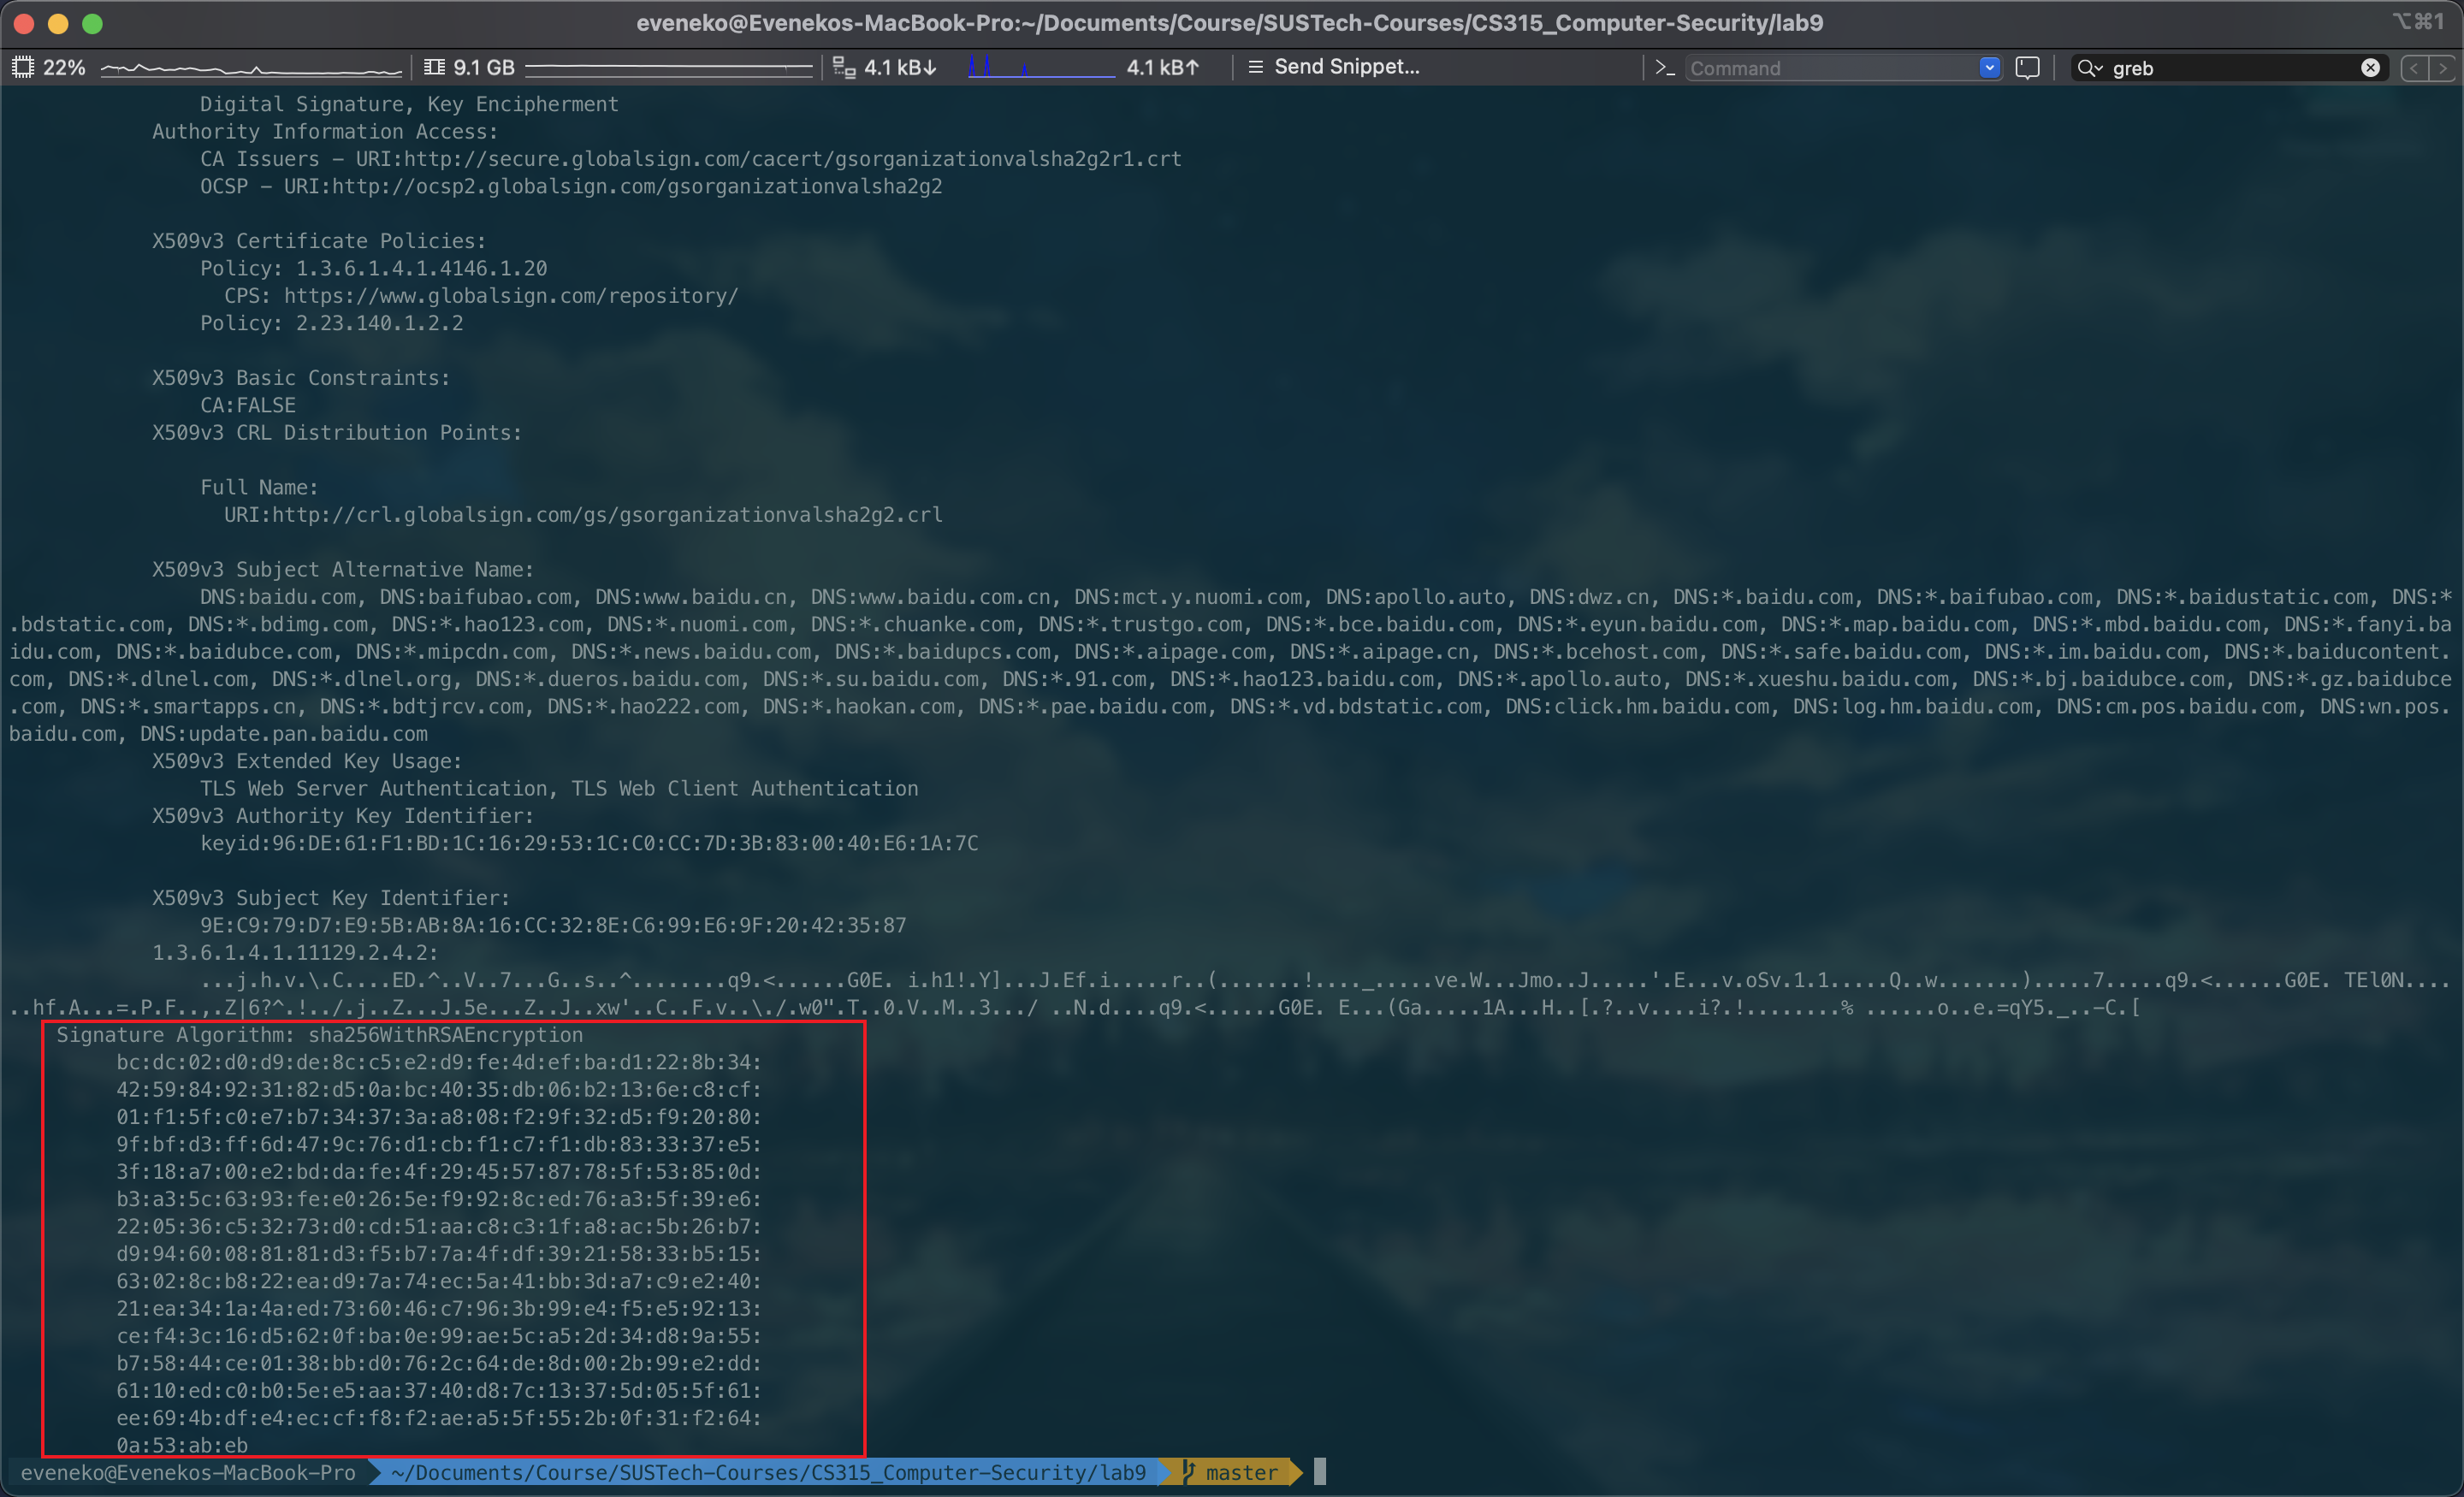
\includegraphics[width=0.85\textwidth]{img/task6_5.png}
    \caption{Step 3}
  \end{figure}

  \begin{figure}[H]
    \centering
    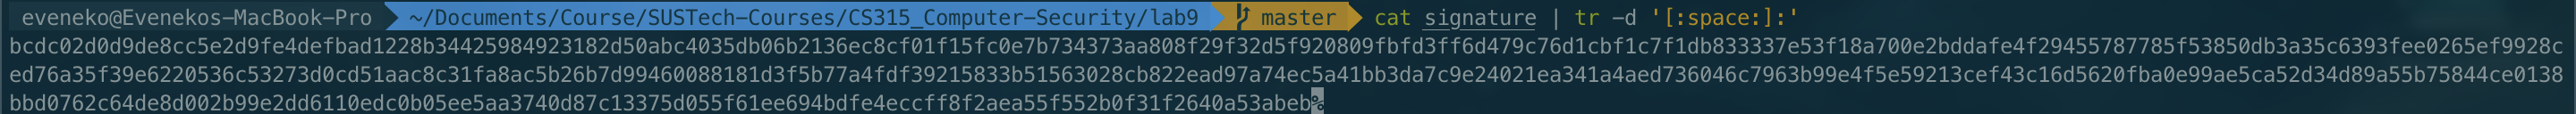
\includegraphics[width=0.85\textwidth]{img/task6_6.png}
    \caption{Step 3}
  \end{figure}

  \subsection*{Step 4}

  Extract the body of the server’s certificate.

  We have $sha256sum$.

  \begin{figure}[H]
    \centering
    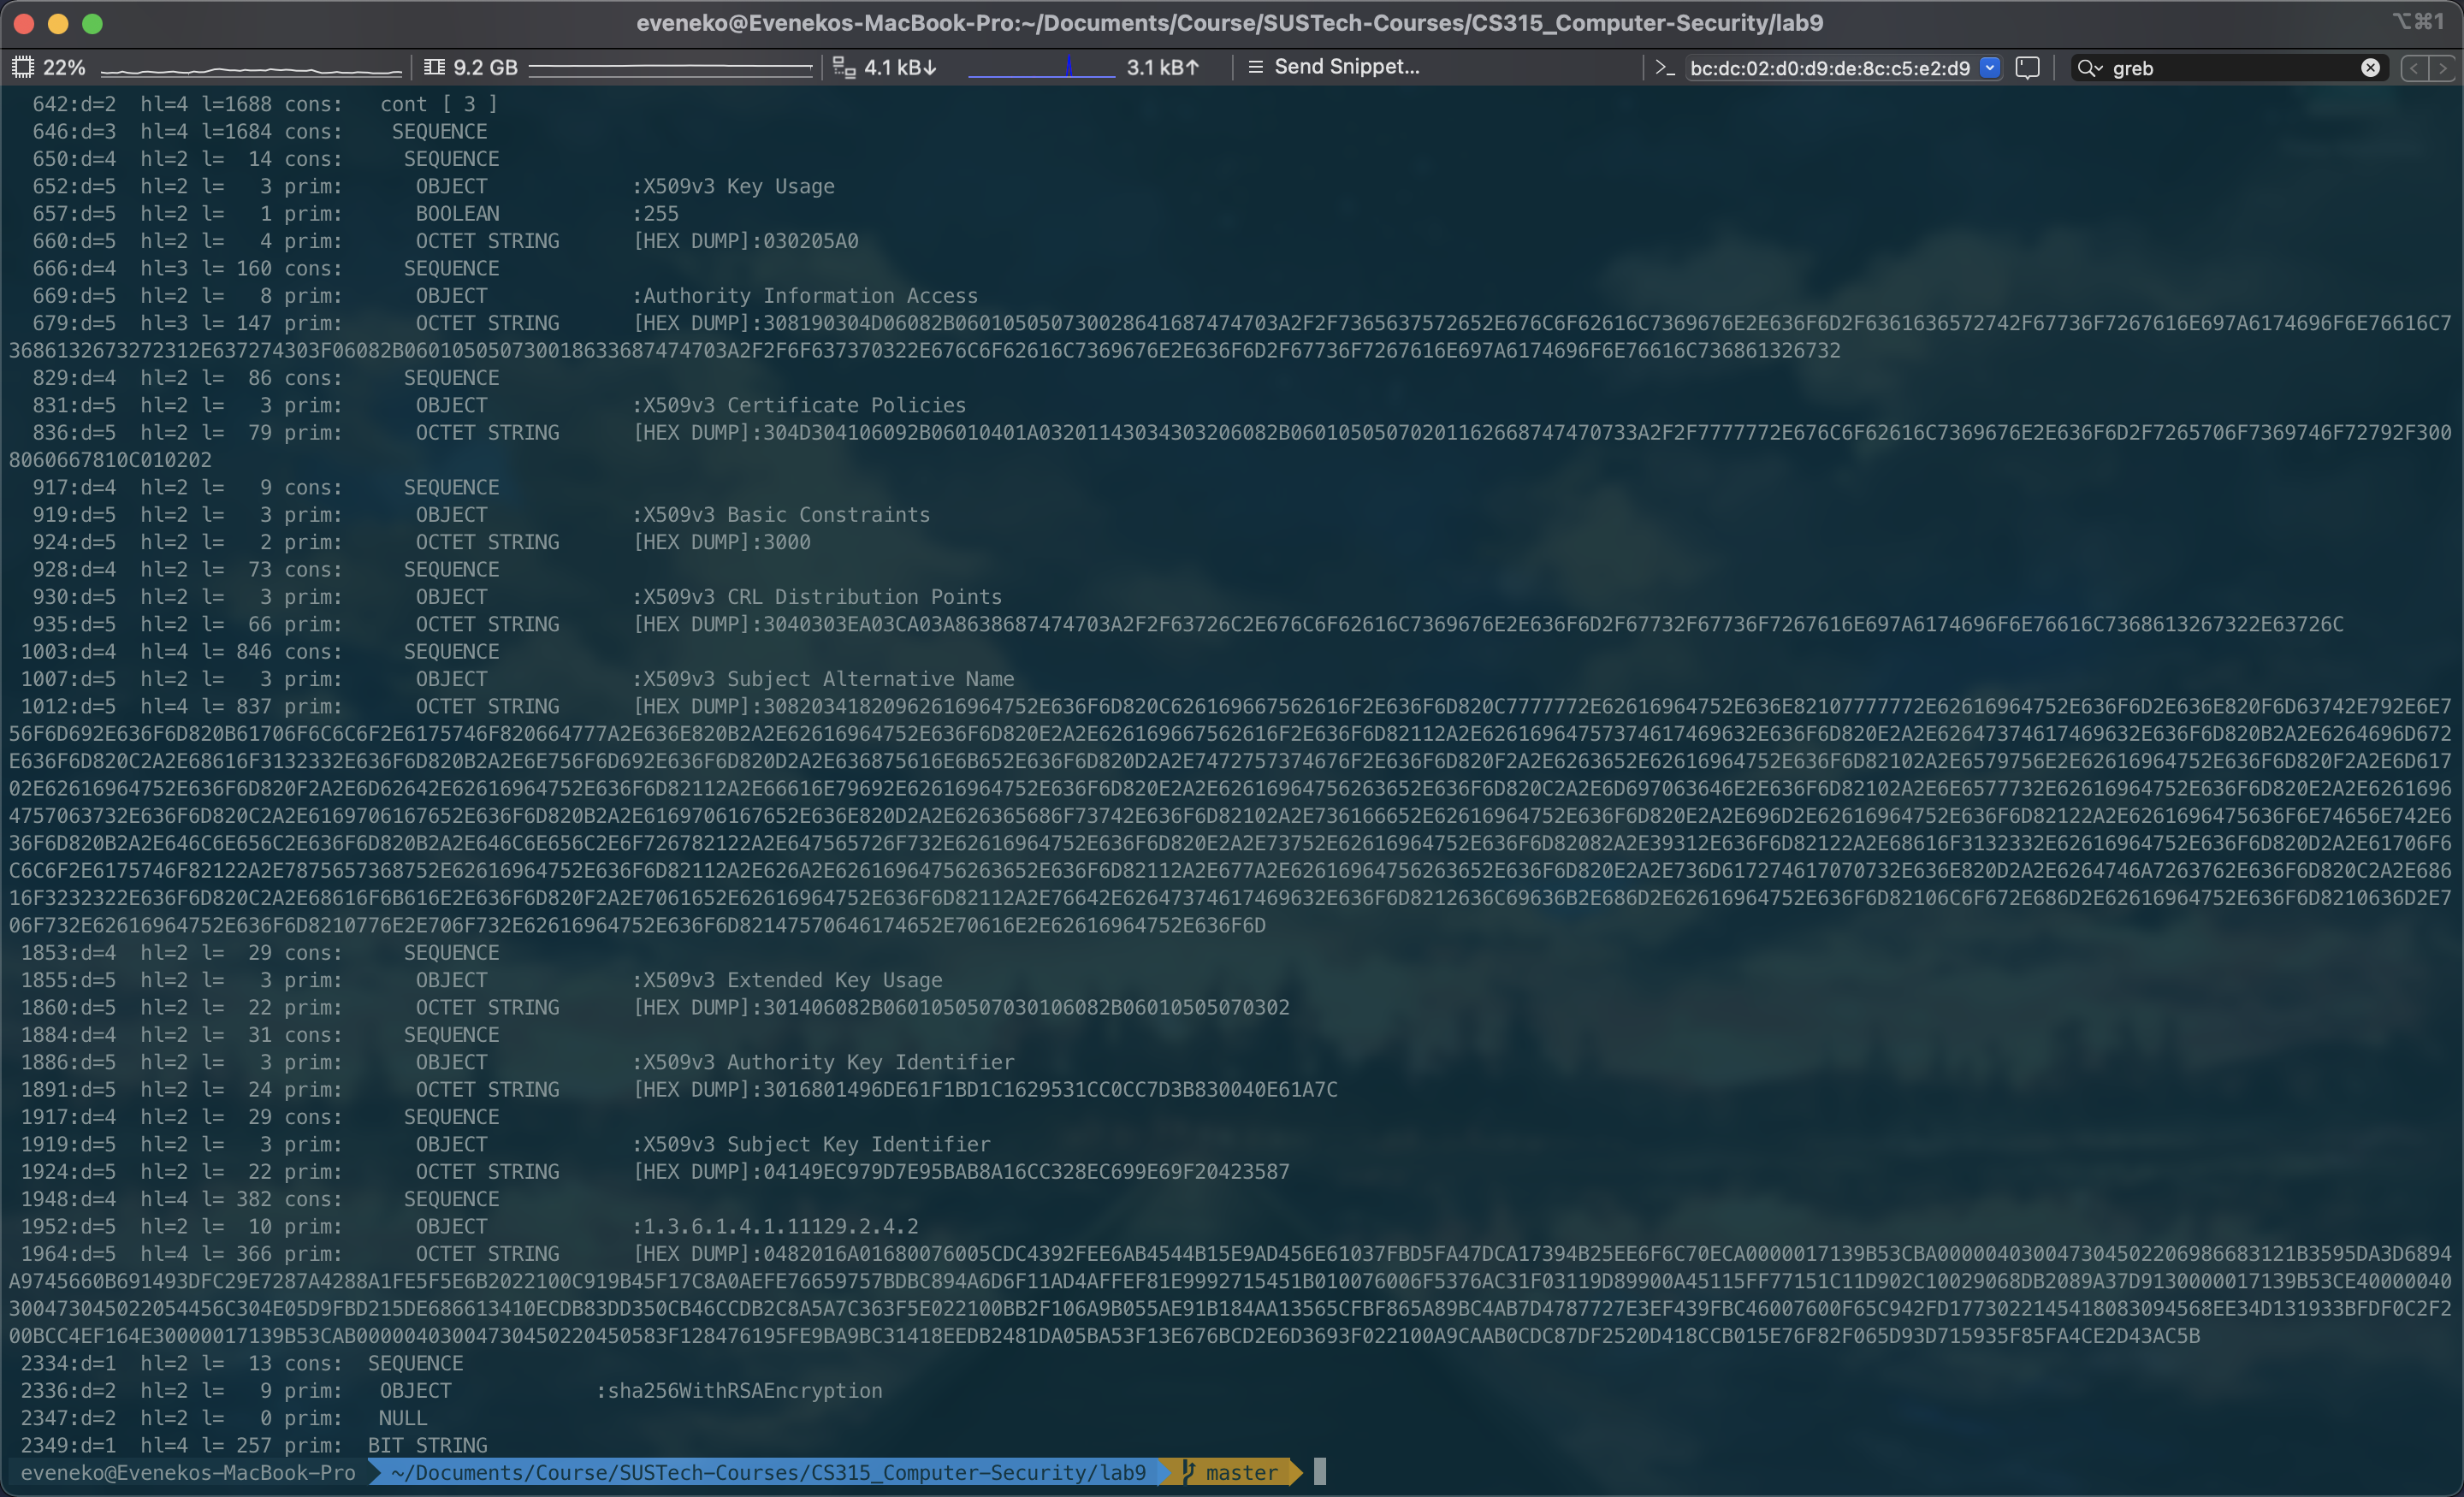
\includegraphics[width=0.85\textwidth]{img/task6_7.png}
    \caption{Step 4}
  \end{figure}

  \begin{figure}[H]
    \centering
    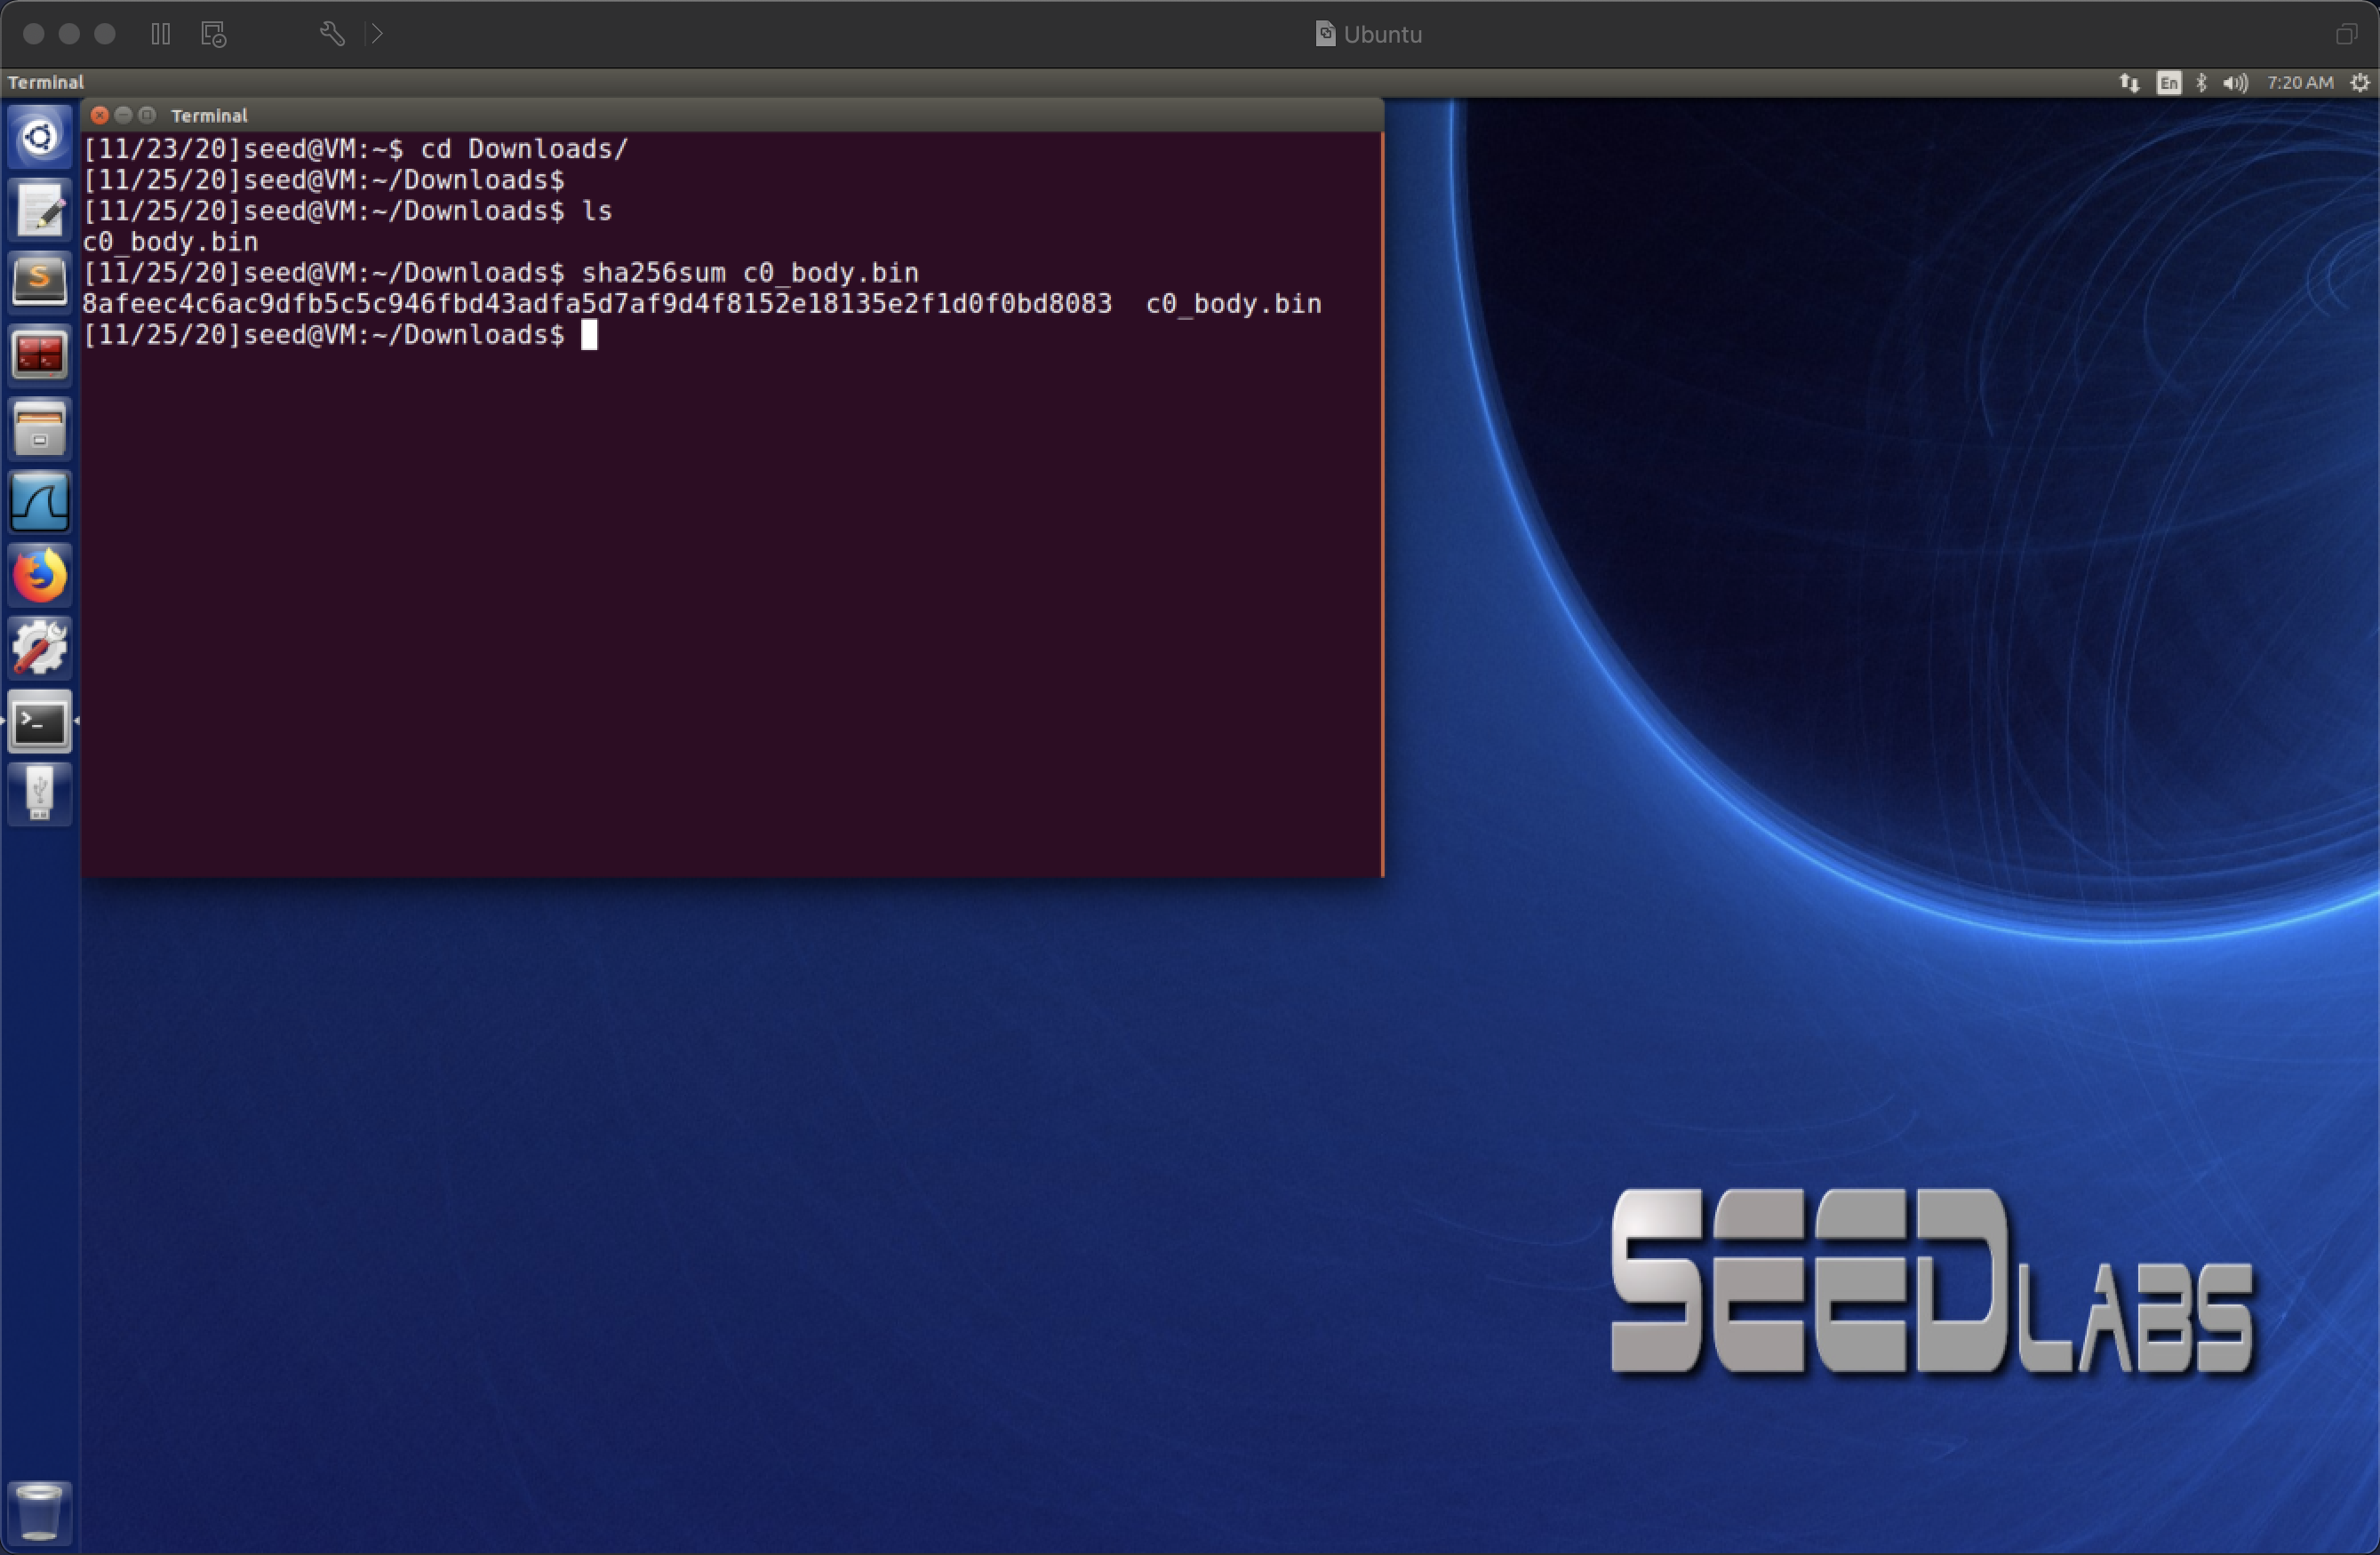
\includegraphics[width=0.85\textwidth]{img/task6_8.png}
    \caption{Step 4}
  \end{figure}

  \subsection*{Step 5}

  Verify the signature.

  We find that the signature $s$ is the same as the result.

  \begin{figure}[H]
    \centering
    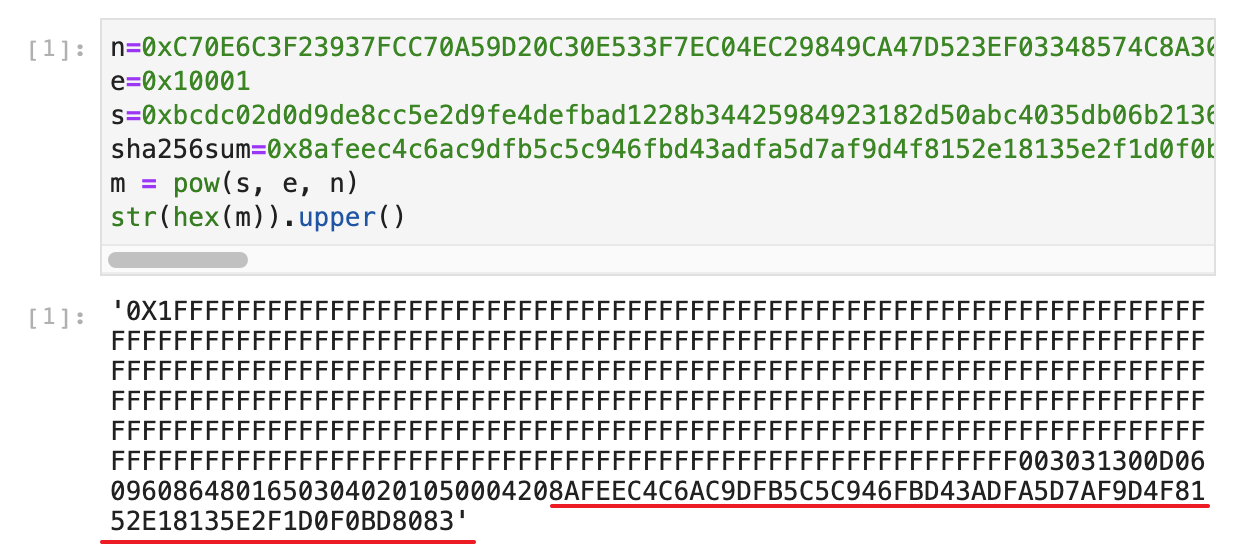
\includegraphics[width=0.85\textwidth]{img/task6_9.png}
    \caption{Step 5}
  \end{figure}

\end{document}
